\begin{frame}{Motivation}
\begin{itemize}
\item We estimated parameters $\theta$  by evaluating the posterior $\mathcal{L}(\theta|y^T)$
\item But we never formally verified whether all elements of $\theta$ are properly identified
\item Parameter identification
\begin{itemize}
  \item is a regularity condition
 \item can and should be assessed before taking your model to data
 \item is a model property
\end{itemize}
\end{itemize}

\end{frame}

\section{The Problem}
\renewcommand{\Source}{\textcite{Cochrane2011}}
\begin{frame}{Simple Example}
\begin{itemize}
\item Consider simple monetary model without price rigidities and real shocks
\item Real interest $r$ is fixed at steady-state level
\item Inflation $\pi_t$ is determined via Fisher equation and central bank reaction function that determines nominal interest rate $i_t$:
\begin{align}
  {i_t} = r + {E_t}{\pi _{t + 1}} \hfill \\
  {i_t} = r + \phi {\pi _t} + {\nu _t} \label{eq:Taylorrule}
\end{align}
\item The two equations imply
\be
{E_t}{\pi _{t + 1}} = \phi {\pi _t} + {\nu _t} \label{eq:cochraneFOC}
\end{equation}
\item We need $ \phi>1$ (\highlight{Taylor-principle}) for Blanchard-Kahn conditions to be satisfied
\item Otherwise: indeterminacy
\end{itemize}
\end{frame}


\begin{frame}{Solution and Estimation}
\begin{itemize}
\item Assume error term is serially correlated (interest smoothing, policy mistakes, etc.) \vspace{-.2cm}
\begin{equation}
{\nu _t} = \rho {\nu _{t - 1}} + {\varepsilon _t}
\end{equation}
\item Iterate equation \eqref{eq:cochraneFOC} forward:
\begin{align}
  {\pi _t} &=  - \sum\nolimits_{j = 0}^\infty  {{{\left( {\frac{1}{\phi }} \right)}^{j + 1}}{E_t}{\nu _{t + j}}}  =  - \frac{1}{{\phi  - \rho }}{\nu _t} \notag \\
   &=  - \frac{1}{{\phi  - \rho }}\left( {\rho {\nu _{t - 1}} + {\varepsilon _t}} \right) = \rho {\pi _{t - 1}} - \frac{{{\varepsilon _t}}}{{\phi  - \rho }} = \rho {\pi _{t - 1}} + {w_t}
\end{align}
where $w_t$ is the new error term ($\varepsilon _t$ and $\nu_t$ not observed)
\item In equilibrium, the nominal interest rate is given by \vspace{-.2cm}
\begin{equation}
{i_t} = r + {E_t}{\pi _{t + 1}} = r + \rho {\pi _t}
\end{equation}
\item Regression of \eqref{eq:Taylorrule} will not estimate $\phi$, but autocorrelation $\rho$
\item Reason: inflation and policy shock $\nu_t$ are perfectly correlated to assure unique stable solution
\item Central bank reaction describes off-equilibrium behavior, it cannot be identified from equilibrium observations!
\end{itemize}
\end{frame}

\renewcommand{\Source}{}
\begin{frame}{The Likelihood Function}
\begin{itemize}
\item Remember: Likelihood function is a \highlight{sufficient statistic}
\item The likelihood function in this case is given by
  \begin{equation}
 \log \left( {f\left( {{\pi _t}|{\pi ^{t - 1}}} \right)} \right) =  - \frac{1}{2}\log \left( {2\pi } \right) - \frac{1}{2}\log \left( {\sigma _{{w_t}}^2} \right) - \frac{1}{2}\frac{{{{\left( {{\pi _t} - \rho {\pi _{t - 1}}} \right)}^2}}}{{\sigma _{{w_t}}^2}}
  \end{equation}
  where
  \begin{equation}
  \sigma _{{w_t}}^2 = {\left( {\frac{{{\sigma _\varepsilon }}}{{\phi  - \rho }}} \right)^2}
  \end{equation}
\item $\rho$ and $\sigma _{{w_t}}$ enter the likelihood function independently from each other and can be estimated
\end{itemize}
\end{frame}

\begin{frame}{Likelihood Plot for $\rho$ and $\sigma _{{w_t}}$}
\begin{figure}
  \includegraphics[scale=.45]{Identification/identifiable}
\end{figure}
\begin{itemize}
\item[] The likelihood function shows a clear peak in $\rho$ and $\sigma _{{w_t}}$
\end{itemize}
\end{frame}

\begin{frame}{Estimating the Components of $\sigma _{{w_t}}$}
\begin{itemize}
\item But: $\sigma _\varepsilon$ and $\phi$ enter multiplicatively and cannot be disentangled
\begin{align}
  \frac{{\partial \log \left( {f\left( {{\pi _t}|{\pi ^{t - 1}}} \right)} \right)}}{{\partial {\sigma _\varepsilon }}} &= \frac{{\partial \log \left( {f\left( {{\pi _t}|{\pi ^{t - 1}}} \right)} \right)}}{{\partial {\sigma _{{w_t}}}}}\frac{{\partial {\sigma _{{w_t}}}}}{{\partial {\sigma _\varepsilon }}} \notag \\
   &= \frac{{\partial \log \left( {f\left( {{\pi _t}|{\pi ^{t - 1}}} \right)} \right)}}{{\partial {\sigma _{{w_t}}}}}\frac{1}{{\phi  - \rho }} \hfill \label{eq:partial_likelihood} \\
  \frac{{\partial \log \left( {f\left( {{\pi _t}|{\pi ^{t - 1}}} \right)} \right)}}{{\partial \phi }} &= \frac{{\partial \log \left( {f\left( {{\pi _t}|{\pi ^{t - 1}}} \right)} \right)}}{{\partial {\sigma _{{w_t}}}}}\frac{{\partial {\sigma _{{w_t}}}}}{{\partial \phi }}  \notag \\
  &=\frac{{\partial \log \left( {f\left( {{\pi _t}|{\pi ^{t - 1}}} \right)} \right)}}{{\partial {\sigma _{{w_t}}}}}\frac{{{\sigma _\varepsilon }}}{{{{\left( {\phi  - \rho } \right)}^2}}}\left( { - 1} \right) \notag\\
  &\stackrel{\eqref{eq:partial_likelihood}}{=}  - \frac{{{\sigma _\varepsilon }}}{{\phi  - \rho }}\frac{{\partial \log \left( {f\left( {{\pi _t}|{\pi ^{t - 1}}} \right)} \right)}}{{\partial {\sigma _\varepsilon }}}
\end{align}
\item The partial derivatives are linearly dependent and the Jacobian is thus singular
\end{itemize}
\end{frame}


\begin{frame}{Likelihood Plot for $\sigma _\varepsilon$ and $\phi$}
\begin{figure}
  \includegraphics[scale=.45]{Identification/non_identifiable}
\end{figure}
\begin{itemize}
\item[] The likelihood function has no unique maximum in $\sigma _\varepsilon$ and $\phi$, only a range of maxima
\end{itemize}
\end{frame}


\renewcommand{\Source}{\textcite{CanovaSala2009}}
\begin{frame}{Identification Problems}
\begin{enumerate}
\item \highlight{Observational Equivalence}: mapping between structural parameters and objective function has no unique maximum
\item[$\Rightarrow$] structural models with potentially different economic interpretations may be indistinguishable
\item \highlight{Under-identification}: objective function is independent of certain structural parameters, e.g.\ because they disappear from rational expectations solution
\item[$\Rightarrow$] \highlight{partial identification} with two structural parameters entering objective function only proportionally, making them separately unrecoverable, is a special case
\item \highlight{weak identification}: parameter theoretically identified, but curvature may be small in certain regions of the parameter space
\end{enumerate}
\end{frame}


\section{Local Identification}

\renewcommand{\Source}{\textcite{Iskrev2010}}
\begin{frame}{State Space System: Transition Equation}
\begin{itemize}
\item Is there a systematic way to detect such issues for elements of $\theta$?
\item Consider generic log-linearized model in state-space form where $\hat x_t=\log(x_t)-\log(x)$
\begin{equation}
  \hat x_{t + 1} = F(\theta) \hat x_t + w_{t + 1},\; w_{t + 1}\mathop  \sim \limits^{iid} \mathcal{N}\left(0,Q(\theta)\right)
\end{equation}
with
\[
Q=CC'
\]
\item Define the vector
\begin{equation}
\tau=\left[\tau_x',\tau_F',\tau_\Omega' \right]
\end{equation}
as the collection of non-constant elements of $\log(x),vec(F)$, and $vech(Q)$, respectively, that depend on $\theta$
\item Drops, e.g., steady states that are always zero or calibrated values
\item The unconditional first and second moments are given by:
\[\begin{gathered}
  E\left( {{{\hat x}_t}} \right) = 0 \hfill \\
  E\left( {{{\hat x}_t}{{\hat x}_t}'} \right) \equiv {\Sigma _x(0)} = F{\Sigma _x}F' + Q \hfill \\
\end{gathered} \]
\end{itemize}
\end{frame}

\begin{frame}{State Space System: Observation Equation}
\begin{itemize}
\item The observables are given by
\begin{equation}
  y_t = H(\theta)x + H(\theta)\hat x_t + \nu_t, \; \nu _t\mathop  \sim \limits^{iid} N\left(0,R(\theta) \right)
\end{equation}
\item In general, only observing $y_t$ would be insufficient to fully characterize the distribution of $x_t$
\item Fortunately, our model implies restrictions through $\theta$
\end{itemize}
\end{frame}


\begin{frame}{The Likelihood Function}
\begin{itemize}
\item The unconditional first and second moments of the observables $y_t$ are given by:
\[\begin{gathered}
  E\left(y_t\right) \equiv {\mu _Y} = H\left( \theta  \right)x \hfill \\
  \operatorname{cov} \left( {{y_{t + i}},{y_t}} \right) \equiv {\Sigma _Y}\left( i \right) = \left\{ {\begin{array}{*{20}{c}}
  {C{\Sigma _x}\left( 0 \right)C' \text{ if } i = 0} \\
  {C{F^i}{\Sigma _x}\left( 0 \right)C' \text{ if } i > 0}
\end{array}} \right. \hfill \\
\end{gathered} \]
\item Stack the unique elements of ${\Sigma _Y}\left( i \right), \: i =\{0,\ldots,T-1\}$ into a vector:
\begin{equation}
{\sigma _Y} = \left[ {vech\left( {{\Sigma _Y}\left( 0 \right)} \right),vec\left( {{\Sigma _Y}\left( 1 \right)} \right), \ldots ,vec\left( {{\Sigma _Y}\left( {T - 1} \right)} \right)} \right]
\end{equation}
and define the vector of first and second moments as
\begin{equation}
{m_T} = [{\mu _Y};{\sigma _Y}] \label{eq:moment_vector}
\end{equation}
\end{itemize}
\end{frame}

\begin{frame}{Definitions}
\begin{definition}[Global Identification]
  Let $\theta\subseteq \Theta \subset \mathcal{R}^k$ be the parameter vector of interest and suppose inference about it is made based on $T$ observations of a random vector $y$ with known joint probability density function $f(Y^T|\theta)$. A point $\theta_0 \in \Theta$ is \highlight{globally identified} if
  \begin{equation}
  f\left( {{Y^T}|\tilde \theta } \right) = f\left( {{Y^T}|{\theta _0}} \right) \text{ with probability 1 } \Rightarrow \tilde \theta  = {\theta _0} \label{eq:global_ident}
  \end{equation}
  for any $\tilde \theta \in \Theta$
\end{definition}
\begin{definition}[Local Identification]
  If Equation \eqref{eq:global_ident} only holds in an open neighborhood of $\theta_0$, then $\theta_0$ is \highlight{locally identified}
\end{definition}
\end{frame}

\begin{frame}{Which Moments?}
\begin{itemize}
\item Typically, the distribution is unknown or assumed to be normal
\item People often use the first two moments
\item Higher order moments might provide additional information \parencite[see e.g.][]{FV2007}
\item Thus, identification based on mean and (co)-variances is sufficient, but not necessary
\end{itemize}
\end{frame}

\begin{frame}{Identification Condition}
\begin{theorem}[Identification Condition]
  Suppose our model in state-space form with $\theta_0$ is the data generating process for $Y^T$. Then $\theta_0$ is \highlight{globally identified} if
  \begin{equation}
  {m_T}\left( {\tilde \theta } \right) = {m_T}\left( {{\theta _0}} \right) \Leftrightarrow \tilde \theta  = {\theta _0}
  \end{equation}
  for any $\tilde \theta \in \Theta$ (and correspondingly for local identification).
\end{theorem}
\begin{itemize}
\item Requires mapping from population moments ${m_T}$ to $\theta$ to be unique
\item If not satisfied, there exists parameter values that imply the same joint distribution
\item[$\Rightarrow$] Even with infinitely many observations, the true value could not be identified
\item Checking global identification is hard $\Rightarrow$ check local identification for relevant parameter range
\end{itemize}
\end{frame}


\begin{frame}{Identification Condition}
\begin{theorem}[Identification Condition]
  Suppose $m_T$ is continuously differentiable function of $\theta$. Then $\theta_0$ is locally identifiable if the Jacobian matrix
  \begin{equation}
  J(q) \equiv \frac{{\partial {m_q}}}{{\partial \theta '}} \label{eq:Jacobian}
  \end{equation}
  has full column rank at $\theta_0$ for $q\leq T$
\end{theorem}
\begin{proof}
  Follows from implicit function theorem.
\end{proof}
\begin{itemize}
\item We need at least as many moments as parameters
\item For sufficient and necessary conditions see the paper
\end{itemize}
\end{frame}

\begin{frame}{Identification Condition: Intuition}

\begin{witemize}
\item Identification requires unique (injective) mapping from structural parameters to population moments
\item Check injectivity by looking at rank of Jacobian matrix
\item One would have to check this condition everywhere $\Rightarrow$ impossible
\item Nevertheless helpful in detecting observational equivalence (column of zeros) and underidentification (linear dependence of columns)
\end{witemize}
\end{frame}


\begin{frame}{Computing the Jacobian}
\begin{itemize}
\item Numerical differentiation and checking for singularity of the numerical Jacobian is prone to numerical errors when functions are nonlinear
\item[$\Rightarrow$] Use analytical derivatives
\item Using the chain rule, the Jacobian in equation \eqref{eq:Jacobian} can be written as
\begin{equation}
J(T) \equiv \underbrace {\frac{{\partial {m_T}}}{{\partial \tau '}}}_{{J_1}\left( T \right)}\underbrace {\frac{{\partial \tau }}{{\partial \theta '}}}_{{J_2}\left( T \right)} \label{eq:Jacobian_chain}
\end{equation}
\item \textcite{Iskrev2010} details how the two parts of the Jacobian can be computed, but we take Dynare's implementation
\item Full rank is often achieved for $q\ll T$: Dynare starts at $q=5$ and increases it if necessary
\end{itemize}
\end{frame}

\begin{frame}{Computing the Jacobian}
\begin{itemize}
\item[]
\begin{equation}
J(T) \equiv \underbrace {\frac{{\partial {m_T}}}{{\partial \tau '}}}_{{J_1}\left( T \right)}\underbrace {\frac{{\partial \tau }}{{\partial \theta '}}}_{{J_2}\left( T \right)} \tag{\ref{eq:Jacobian_chain}}
\end{equation}
\item ${J_2}\left( T \right)$ shows how the parameters $\theta$ affect the non-constant model solution parts $\tau$
\item ${J_1}\left( T \right)$ shows how the model solution maps into the observed data moments
\end{itemize}
\begin{corollary}
  The point $\theta_0$ is locally identifiable only if $J_2(T)$ has full rank
\end{corollary}
\begin{itemize}
\item Necessary condition as parameters only affect distribution of observables through their effect on model solution
\item It is not sufficient unless all states are observed
\item ${{J_1}\left( T \right)}$ provides information on whether a theoretically identifiable parameter can be identified using the observables contained in $y$
\end{itemize}
\end{frame}

\begin{frame}{Dynare Output for the Cochrane Toy Model}
\begin{figure}
  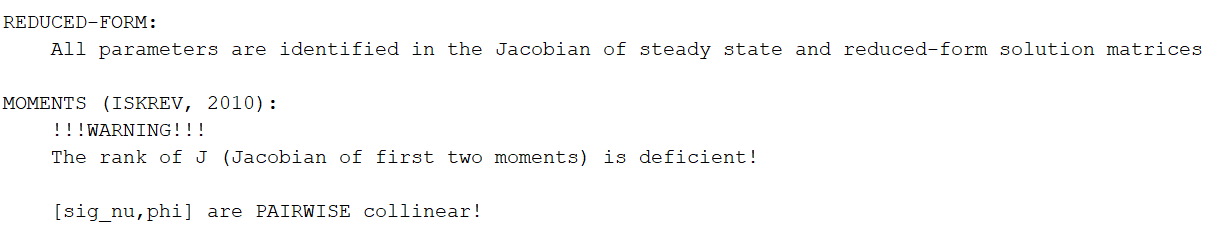
\includegraphics[scale=.45]{Figures/dynare_toy_cochrane}
\end{figure}
\begin{itemize}
\item All parameters are identified in the model
\item However, without observing $\nu_t$, the elements of $\sigma_w$ cannot be disentangled
\end{itemize}
\end{frame}

\begin{frame}{Dynare Output for Our RBC Model}
\begin{figure}
  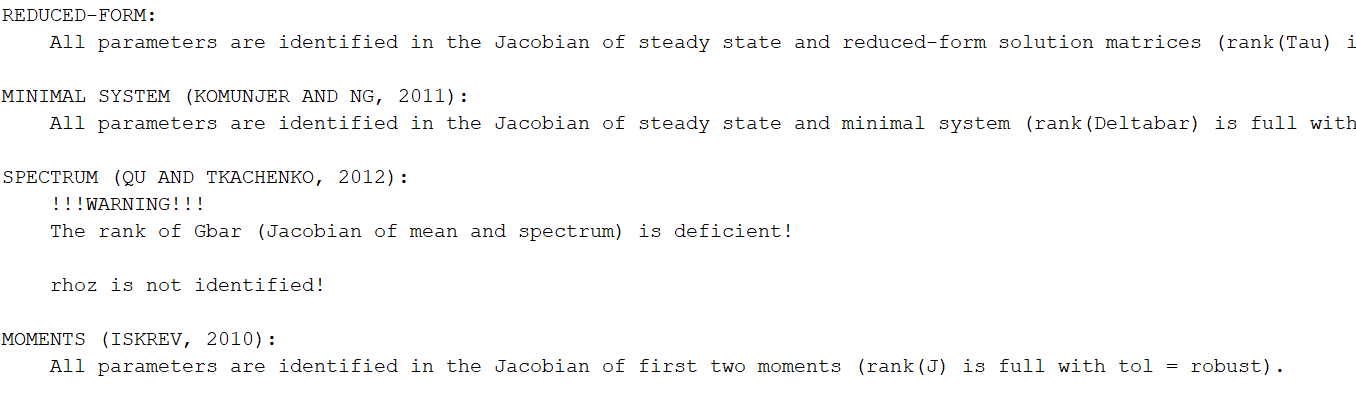
\includegraphics[scale=.45]{Figures/dynare_rbc}
\end{figure}
\begin{itemize}
\item All parameters are identified in the model and using our observables
\end{itemize}
\end{frame}

\section{Spectrum}

\begin{frame}{Diagnostics based on spectrum}

\begin{itemize}
\item State space solution also allows computing theoretical spectral density $\mathcal{S}_{2,x}(\omega)$ and $\mathcal{S}_{2,y}(\omega)$ for $\omega \in [-\pi,\pi]$
\item \textcite{QuTkachenko2012} show that identification implies unique (injective) mapping from structural parameters to population mean and spectral density\\
$\rightarrow$ check injectivity by looking at rank of Jacobian matrix
\item Rank condition: Jacobian of theoretical mean and spectrum of observables w.r.t structural parameters has full rank
\item Again, helpful in detecting observational equivalence (columns of zeros and linear dependence between parameters or try all combinations of sets of parameters);
\item Gram matrix structure numerically facilitates rank computations, no order condition (at least as many moments are parameters) required 
\item Checking global identification is hard, but one can check local identification for relevant parameter range
\end{itemize}
\end{frame}

%\begin{frame}{Minimal State Space System}
%
%\begin{itemize}
%\item State space solution also allows computing minimal state space system with minimal state variables $\tilde x_t$
%\item Dynamics are entirely driven by the smallest possible dimension of the state vector (and shocks)
%\item Definition of minimality:
%\begin{itemize}
%  \item Controllability: For any initial state, it is always possible to design an input sequence that puts
%the system in the desired final state
% \item Observability: Given the evolution of the input it is always possible to reconstruct the initial
%state by observing the evolution of the output
%\end{itemize}
%\item Solution in Dynare is by default not based on the minimal state representation (but there is a
%function \texttt{get\_minimal\_state\_representation.m})
%\item Numerical procedures (pole-zero cancellation) do not necessarily output minimal states with economic meaning
%\end{itemize}
%\end{frame}

\section{Dynare Implementation}
\begin{frame}{\texttt{identification}-command}

\begin{itemize}
\item Triggers the local identification tests and has two modes of operation:
\begin{enumerate}
 \item Point identification check (default)
 \item Monte Carlo mode (e.g. \texttt{prior\_mc=1000})
\end{enumerate}
\item By default all model parameters and all stderr parameters are checked
\item Parameters can be selected with \texttt{estimated\_params} block either with
\begin{enumerate}
\item  initial values
\item  prior information
\end{enumerate}
\end{itemize}
\end{frame}

\begin{frame}{A warning}

\begin{itemize}
\item Identification checks typically require symbolic derivatives to achieve sufficient precision
\item Dynare's symbolic preprocessor interprets and implements the model definitions as expressed in the Dynare file\\
$\rightarrow$ will not reflect all parameter definitions hidden e.g. in a custom \texttt{\_steadystate.m} file \\
$\rightarrow$ use \texttt{steady\_state\_model} block instead)
\item Do not declare auxiliary parameters, rather use model-local variables ('\#' syntax in the
model \texttt{block}) to declare endogenous parameters
\end{itemize}
\end{frame}

\begin{frame}{Tracking singularities}

\begin{itemize}
\item When Jacobians are rank deficient, code tries to diagnose subset of parameters responsible:
\begin{itemize}
  \item ranks are computed using the singular value decomposition
  \item for columns of zeros in Jacobian, associated parameter is printed on command window
  \item compute pairwise- and multi-correlation coefficients for each column of Jacobian\\
  $\rightarrow$ print parameter combinations with correlation coefficients equal to unity
\end{itemize}
\item Alternatively: a brute-force approach to check rank conditions for all possible combinations
can be triggered (\texttt{checks\_via\_subsets=1})
\end{itemize}
\end{frame}

\section{Identification Strength}

\renewcommand{\Source}{\textcite{Iskrev2011}}

\begin{frame}{The Information Matrix Revisited}
\begin{itemize}
    \item The precision of the parameter estimates at the mode was given (asymptotically) by the inverse of the \highlight{Fisher Information Matrix}
    \begin{equation}
    I\left( \theta  \right) = E\left[ {\left( {\frac{{\partial \log \left( {p\left( {Y|\theta } \right)} \right)}}{{\partial \theta '}}} \right)'\left( {\frac{{\partial \log \left( {p\left( {Y|\theta } \right)} \right)}}{{\partial \theta '}}} \right)} \right]
    \end{equation}
    \item Typically, non-singularity of this matrix is sufficient for local identification \parencite[for details see][]{Iskrev2011}
    \item Can be decomposed into a variance matrix $\Delta$ and a correlation matrix $\tilde I\left( \theta  \right)$
    \begin{equation}
    I\left( \theta  \right) = {\Delta ^{\frac{1}{2}}}\tilde I\left( \theta  \right){\Delta ^{\frac{1}{2}}} \label{eq:Fisher_decomposed}
    \end{equation}
    where
    \[
    \Delta  = \text{diag}\left( {I\left( \theta  \right)} \right)
    \]
\end{itemize}
\end{frame}

\begin{frame}{Identification Strength}
\begin{itemize}
    \item[]
    \begin{equation}
    I\left( \theta  \right) = {\Delta ^{\frac{1}{2}}}\tilde I\left( \theta  \right){\Delta ^{\frac{1}{2}}} \tag{\ref{eq:Fisher_decomposed}}
    \end{equation}
    \item Here, we can again see our two reasons for non-identifiability:
    \begin{enumerate}
      \item The likelihood does not change when parameter $i$ changes, i.e.\
      \begin{equation}
      \Delta_i=0
      \end{equation}

      \item The effect on the likelihood is offset due to perfect correlation, i.e.\
      \begin{equation}
      {\rho _i} \equiv corr\left( {\frac{{\partial \log \left( {p\left( {Y|\theta } \right)} \right)}}{{\partial {\theta _i}}},\frac{{\partial \log \left( {p\left( {Y|\theta } \right)} \right)}}{{\partial {\theta _{ - i}}}}} \right) = 1
      \end{equation}
    \end{enumerate}
    \item This suggests that we can use this curvature information also for \highlight{weak identification} as in that case $\Delta_i\approx 0$ and/or $\rho_i\approx1$
\end{itemize}
\end{frame}

\begin{frame}{Identification Strength}
\begin{itemize}
    \item Identification strength can be measured using
    \begin{equation}
    {s_i}\left( \theta  \right) = \sqrt {{\Delta _i}\left( {1 - \rho _i^2} \right)}
    \end{equation}
    \item If $I(\theta)$ is not singular, $1/{s_i}\left( \theta  \right)$ is equal to the square root of the $i$th diagonal element of $(I(\theta))^{-1}$, i.e.
    \begin{equation}
    {s_i}\left( \theta  \right)=\sqrt{\frac{1}{\left(\left(I(\theta)\right)^{-1}\right)_{(ii)}}} \label{eq:sensitivity}
    \end{equation}
    \item As this measure only uses the population objective function (expected log-likelihood), it is an a-priori measure
    \item At the same time, it can be interpreted as the lower bound on the estimation uncertainty in an unbiased finite sample estimator
\end{itemize}
\end{frame}

\begin{frame}{Identification Strength}
\begin{itemize}
    \item Problem: measure is percentage change in likelihood for unit change in parameter $\rightarrow$ not unit free
    \item Solution: multiply with value of $\theta_i$ to obtain elasticity measure:
    \begin{equation}
    s_i^r\left( \theta  \right) = \sqrt {{\theta _i}{\Delta _i}}  \times \sqrt {\left( {1 - \rho _i^2} \right)}
    \end{equation}
    where the first part is the elasticity of the likelihood function w.r.t.\ $\theta_i$, keeping all other parameters constant
\end{itemize}
\end{frame}

\renewcommand{\Source}{\textcite{RattoIskrev2011}}

\begin{frame}{Dynare Implementation}
\begin{itemize}
    \item The strength of identification for parameter $\theta_i$ is defined through a renormalized version of the curvature as
    \begin{equation}
    {s_i^{dyn}} = \theta _i \times s_i(\theta)\overset{\eqref{eq:sensitivity}}{=}\sqrt {\frac{{\theta _i^2}}{{{{\left( {I{{\left( \theta  \right)}^{ - 1}}} \right)}_{\left( {i,i} \right)}}}}} \quad \text[STRENGTH]
    \end{equation}
    \item Can be interpreted as an ``a-priori t-test''
    \item Taking square of $\theta$ assures it to be positive
    \item The \highlight{sensitivity component} contained in this measure (as opposed to the \highlight{correlation component}) is defined as
    \begin{equation}
    {\tilde\Delta _i} =\sqrt {{\theta _i^2}{\Delta _i}}= \sqrt {\theta _i^2I{{\left( \theta  \right)}_{\left( {i,i} \right)}}} \quad \text[SENSITIVITY]
    \end{equation}
    \item Identification is often checked over the prior region, e.g.\ at the prior mean
\end{itemize}
\end{frame}

\begin{frame}{Dynare Implementation}
\begin{itemize}
    \item Because some parameters may have a prior mean of zero, an alternative normalization uses the prior standard deviation $\sigma(\theta_i)$:
    \begin{align}
  {s_i} &= \sqrt {\frac{{{{\left( {\sigma \left( {{\theta _i}} \right)} \right)}^2}}}{{{{\left( {I{{\left( \theta  \right)}^{ - 1}}} \right)}_{\left( {i,i} \right)}}}}}  \quad \text[STRENGTH] \\
  {\tilde \Delta _i} &= \sqrt {{{\left( {\sigma \left( {{\theta _i}} \right)} \right)}^2}I{{\left( \theta  \right)}_{\left( {i,i} \right)}}}  \quad \text[SENSITIVITY]
\end{align} 
\end{itemize}
\end{frame}

\begin{frame}{Dynare Output for Our RBC Model}
\begin{figure}
  \includegraphics[scale=.45]{Identification/RBC_ident/identification/RBC_ident_ident_strength_prior_mean}
\end{figure}
\end{frame}



\section{Advanced Mode}

\begin{frame}{The \texttt{advanced=1} option}
\begin{itemize}
\item Additional analysis of the LRE form (steady-state and dynamic model derivatives) for all model variables
\item Different Sensitivity Measure based on norm of columns of Jacobians
\item Analysis of identification patterns based on regressions and Singular Value Decompositions
\end{itemize}
\end{frame}
Point mode

\begin{frame}{A Different Sensitivity Measure}
\begin{itemize}
\item Another sensitivity measure is how changes in the elements of the parameter vector $\theta$ impact the model moments
\item Can be measured locally using the Jacobian, where the entry $\partial m_j/\partial \theta_i$ needs to be normalized
\item Can be done by multiplying with the ratio of standard deviations
\begin{equation}
\std(\theta_i)/\std(m_j)
\end{equation}
\item Accounts for different parameter uncertainty by ascribing more importance to more variable parameters (effectively normalizing across parameters $i$)
\item Normalization with standard deviation $\std(m_j)$ allows for comparing the impact of parameter $i$ on differently volatile moments (normalizing across moments $j$).
\item Norm of the columns of the standardized Jacobian yields single aggregate sensitivity measure over all moments $j$ for each parameter $i$.
\end{itemize}
\end{frame}

\begin{frame}{Dynare Output for Our RBC Model}
\begin{figure}
  \includegraphics[scale=.45]{Identification/RBC_ident/identification/RBC_ident_sensitivity_prior_mean}
\end{figure}
\begin{itemize}
  \item The respective Jacobian matrices refer to
  \begin{enumerate}
    \item the moments matrix ($\partial m_T/\partial \theta'$), indicating  how well a parameter can be identified due the strength of its impact on the observed moments
    \item the model solution matrices ($\partial \tau/\partial \theta'$), indicating how well a parameter could in principle be identified if all state variables were observed
    \item the Linear Rational Expectations  model ($\partial \gamma/\partial \theta'$), indicating trivial cases of non-identifiability due to e.g.\ some parameters always showing up as a product in the model equations
  \end{enumerate}
\end{itemize}
\end{frame}

\begin{frame}{Correlation Component}
\begin{itemize}
  \item Even if the likelihood itself is sensitive, there might be (perfect) collinearity
  \item Need to look at correlation component
  \item  This analysis is conducted via brute force: For each single parameter, a set of regressions is run of the column of the Jacobian corresponding to the parameter in the row on all possible combinations of other Jacobian columns
  \item Aim: finding the column (and thus parameter) combination with the highest $R^2$
\end{itemize}
\end{frame}

\begin{frame}{Dynare Output for Our RBC Model}
\begin{figure}
  \includegraphics[scale=.45]{Identification/RBC_ident/identification/RBC_ident_ident_collinearity_prior_mean_1}
\end{figure}
\end{frame}

\begin{frame}{Dynare Output for Our RBC Model}
\begin{figure}
  \includegraphics[scale=.45]{Identification/RBC_ident/identification/RBC_ident_ident_collinearity_prior_mean_2}
\end{figure}
\end{frame}

\begin{frame}{Dynare Output for Our RBC Model}
\begin{itemize}
  \item Following \textcite{Andrle2010}, identification can also be judged from a singular value decomposition (SVD) of the information matrix
  \item Provides the size of the singular values and the associated eigenvectors (i.e.\ parameters)
  \item Parameter combinations associated with the smallest singular values are closest to being perfectly collinear and thus redundant
  \item Singular value of 0 implies that the parameter is completely unidentified as it is responsible for the information matrix being rank deficient
\end{itemize}
\end{frame}



\begin{frame}{Dynare Output for Our RBC Model: SVD}
\begin{figure}
  \includegraphics[scale=.45]{Identification/RBC_ident/identification/RBC_ident_ident_pattern_prior_mean_1}
\end{figure}

\end{frame} 